\subsection{System Characteristics}
\label{sec:SystemCharacteristics}

\subsubsection{Steady State}
\label{sub:SteadyState}

The steady state response of the system was determined by setting the duty cycle of the LED to all values in the PWM range 0--255. \textcolor{red}{Each sample was acquired \SI{200}{\milli\second} after the previous one so that the system had time to reach a steady state. This is an adequate time between samples because $RC$ constant of the detector circuit in \autoref{fig:setup_LDR_circuit} is $\tau = R_2C_1 = \SI{60}{\milli\second}$ and \SI{400}{\milli\second} amounts to $3\tau$. The reason why $R_2$ is in the time constant and not $R_3$ is because the PWM value was incremented and hence $C_1$ charges via $R_2$. If the data was acquired while decrementing the PWM value $R_3$ would be used instead.}

% explain R_2's value above?

A graph of the acquired data can be seen in \autoref{fig:steady_state}. We conclude that the resistance of the LDR does not vary linearly with the duty cycle on the LED.

\begin{figure}[h]
    \centering
    \resizebox{\textwidth}{!}{% Title: glps_renderer figure
% Creator: GL2PS 1.3.8, (C) 1999-2012 C. Geuzaine
% For: Octave
% CreationDate: Tue Dec 29 23:09:54 2015
\setlength{\unitlength}{1pt}
\begin{picture}(0,0)
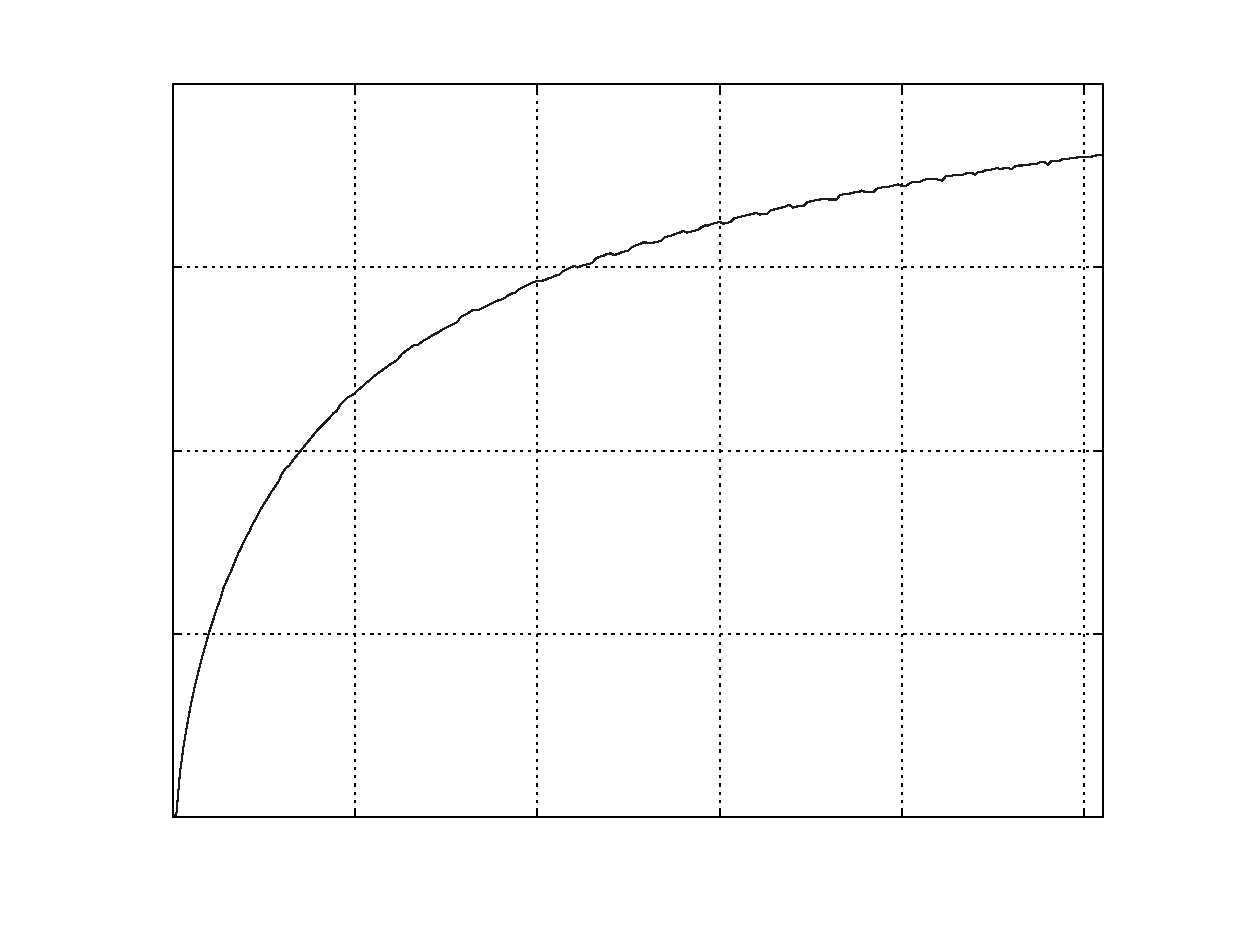
\includegraphics{img/steady_state-inc}
\end{picture}%
\begin{picture}(576,432)(0,0)
\fontsize{10}{0}
\selectfont\put(74.88,42.5189){\makebox(0,0)[t]{\textcolor[rgb]{0,0,0}{{0}}}}
\fontsize{10}{0}
\selectfont\put(162.409,42.5189){\makebox(0,0)[t]{\textcolor[rgb]{0,0,0}{{50}}}}
\fontsize{10}{0}
\selectfont\put(249.939,42.5189){\makebox(0,0)[t]{\textcolor[rgb]{0,0,0}{{100}}}}
\fontsize{10}{0}
\selectfont\put(337.468,42.5189){\makebox(0,0)[t]{\textcolor[rgb]{0,0,0}{{150}}}}
\fontsize{10}{0}
\selectfont\put(424.998,42.5189){\makebox(0,0)[t]{\textcolor[rgb]{0,0,0}{{200}}}}
\fontsize{10}{0}
\selectfont\put(512.527,42.5189){\makebox(0,0)[t]{\textcolor[rgb]{0,0,0}{{250}}}}
\fontsize{10}{0}
\selectfont\put(69.8755,47.52){\makebox(0,0)[r]{\textcolor[rgb]{0,0,0}{{0}}}}
\fontsize{10}{0}
\selectfont\put(69.8755,135.54){\makebox(0,0)[r]{\textcolor[rgb]{0,0,0}{{1}}}}
\fontsize{10}{0}
\selectfont\put(69.8755,223.56){\makebox(0,0)[r]{\textcolor[rgb]{0,0,0}{{2}}}}
\fontsize{10}{0}
\selectfont\put(69.8755,311.58){\makebox(0,0)[r]{\textcolor[rgb]{0,0,0}{{3}}}}
\fontsize{10}{0}
\selectfont\put(69.8755,399.6){\makebox(0,0)[r]{\textcolor[rgb]{0,0,0}{{4}}}}
\fontsize{10}{0}
\selectfont\put(298.08,31.5188){\makebox(0,0)[t]{\textcolor[rgb]{0,0,0}{{PWM value (0--255)}}}}
\fontsize{10}{0}
\selectfont\put(59.8755,223.56){\rotatebox{90}{\makebox(0,0)[b]{\textcolor[rgb]{0,0,0}{{Voltage at \texttt{A0} (\si{\volt})}}}}}
\end{picture}
}
    \caption{Steady state voltage at pin \texttt{A0} as a function of the duty cycle of the LED}
    \label{fig:steady_state}
\end{figure}

\subsubsection{Step Response}
\label{sub:StepResponse}

\begin{figure}[h]
    \centering
    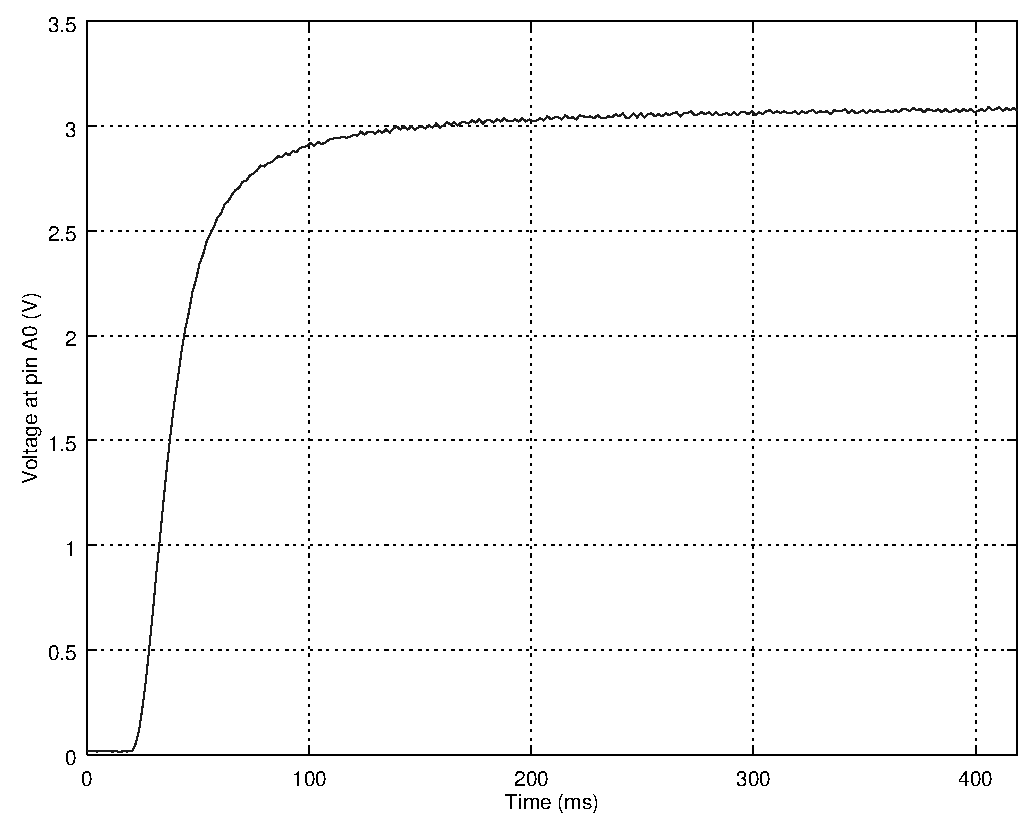
\includegraphics[width=.85\textwidth]{img/step_response}
    \caption{}
    \label{fig:step_response}
\end{figure}

\subsubsection{Incremental Response}
\label{sub:IncrementalResponse}

\subsubsection{Modeling the LDR}
\label{subsubsec:LDR_model}

\begin{figure}[h]
    \centering
    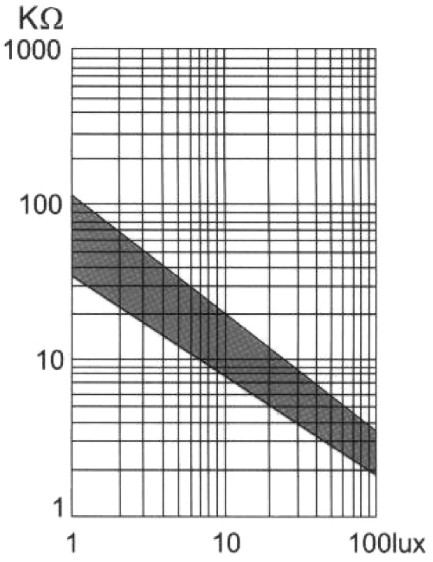
\includegraphics[width=.4\textwidth]{img/LDR_datasheet}
    \caption{}
    \label{fig:LDR_datasheet}
\end{figure}

\begin{figure}[h]
    \centering
    \resizebox{\textwidth}{!}{% Title: glps_renderer figure
% Creator: GL2PS 1.3.8, (C) 1999-2012 C. Geuzaine
% For: Octave
% CreationDate: Tue Dec 29 00:54:08 2015
\setlength{\unitlength}{1pt}
\begin{picture}(0,0)
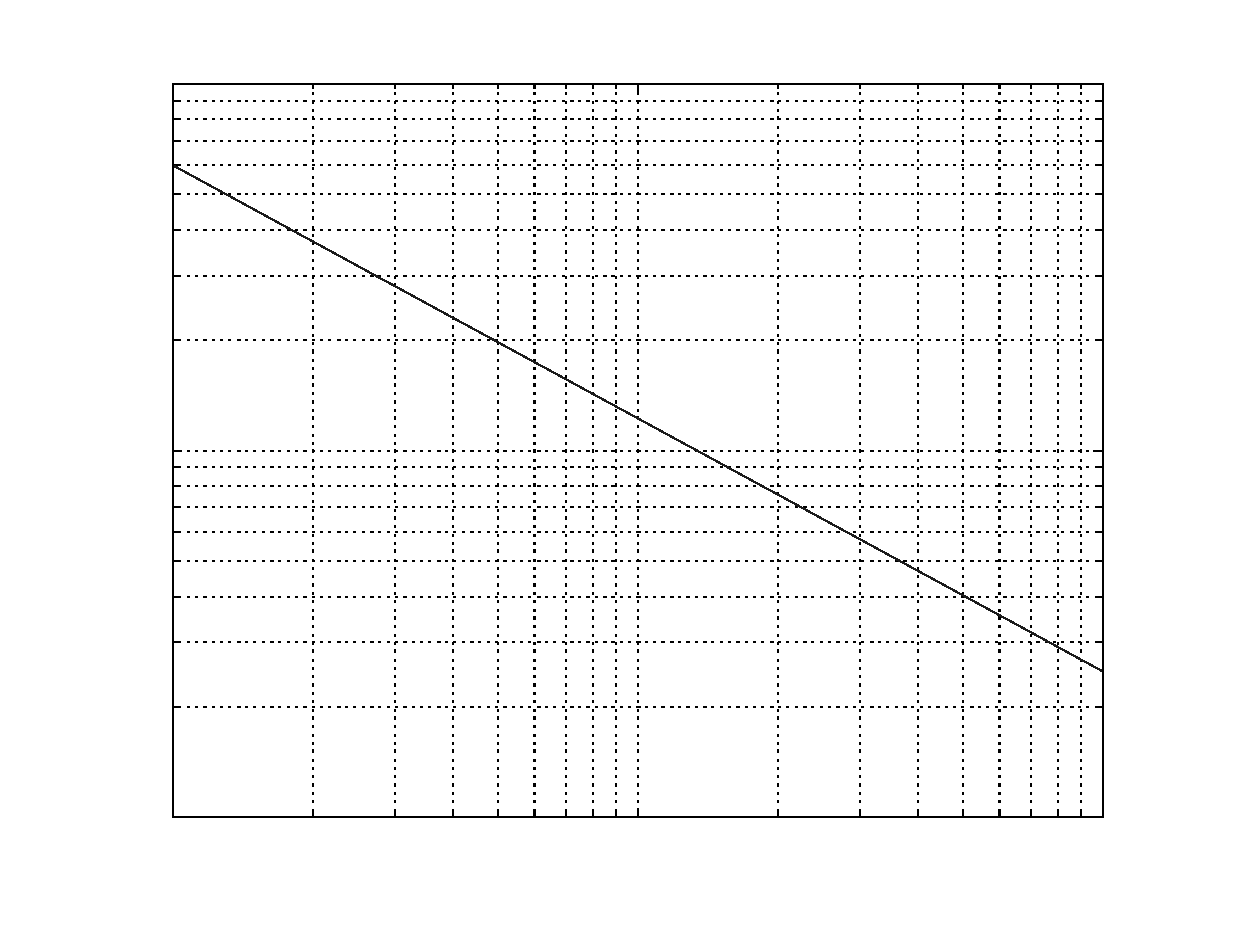
\includegraphics{img/LDR_model-inc}
\end{picture}%
\begin{picture}(576,432)(0,0)
\fontsize{10}{0}
\selectfont\put(74.88,42.5189){\makebox(0,0)[t]{\textcolor[rgb]{0,0,0}{{1e+0}}}}
\fontsize{10}{0}
\selectfont\put(298.08,42.5189){\makebox(0,0)[t]{\textcolor[rgb]{0,0,0}{{1e+1}}}}
\fontsize{10}{0}
\selectfont\put(521.28,42.5189){\makebox(0,0)[t]{\textcolor[rgb]{0,0,0}{{1e+2}}}}
\fontsize{10}{0}
\selectfont\put(69.8755,47.52){\makebox(0,0)[r]{\textcolor[rgb]{0,0,0}{{1e+3}}}}
\fontsize{10}{0}
\selectfont\put(69.8755,223.56){\makebox(0,0)[r]{\textcolor[rgb]{0,0,0}{{1e+4}}}}
\fontsize{10}{0}
\selectfont\put(69.8755,399.6){\makebox(0,0)[r]{\textcolor[rgb]{0,0,0}{{1e+5}}}}
\fontsize{10}{0}
\selectfont\put(298.08,31.5188){\makebox(0,0)[t]{\textcolor[rgb]{0,0,0}{{Illuminance (\si{\lux})}}}}
\fontsize{10}{0}
\selectfont\put(39.8755,223.56){\rotatebox{90}{\makebox(0,0)[b]{\textcolor[rgb]{0,0,0}{{Resistance (\si{\ohm})}}}}}
\end{picture}
}
    \caption{Resistance of the LRD as function of the incident illuminance}
    \label{fig:LDR_model}
\end{figure}

\subsubsection{LDR to Lux}
\label{sub:LDRtoLux}

\begin{figure}[h]
    \centering
    \resizebox{\textwidth}{!}{% Title: glps_renderer figure
% Creator: GL2PS 1.3.8, (C) 1999-2012 C. Geuzaine
% For: Octave
% CreationDate: Mon Dec 28 19:17:53 2015
\setlength{\unitlength}{1pt}
\begin{picture}(0,0)
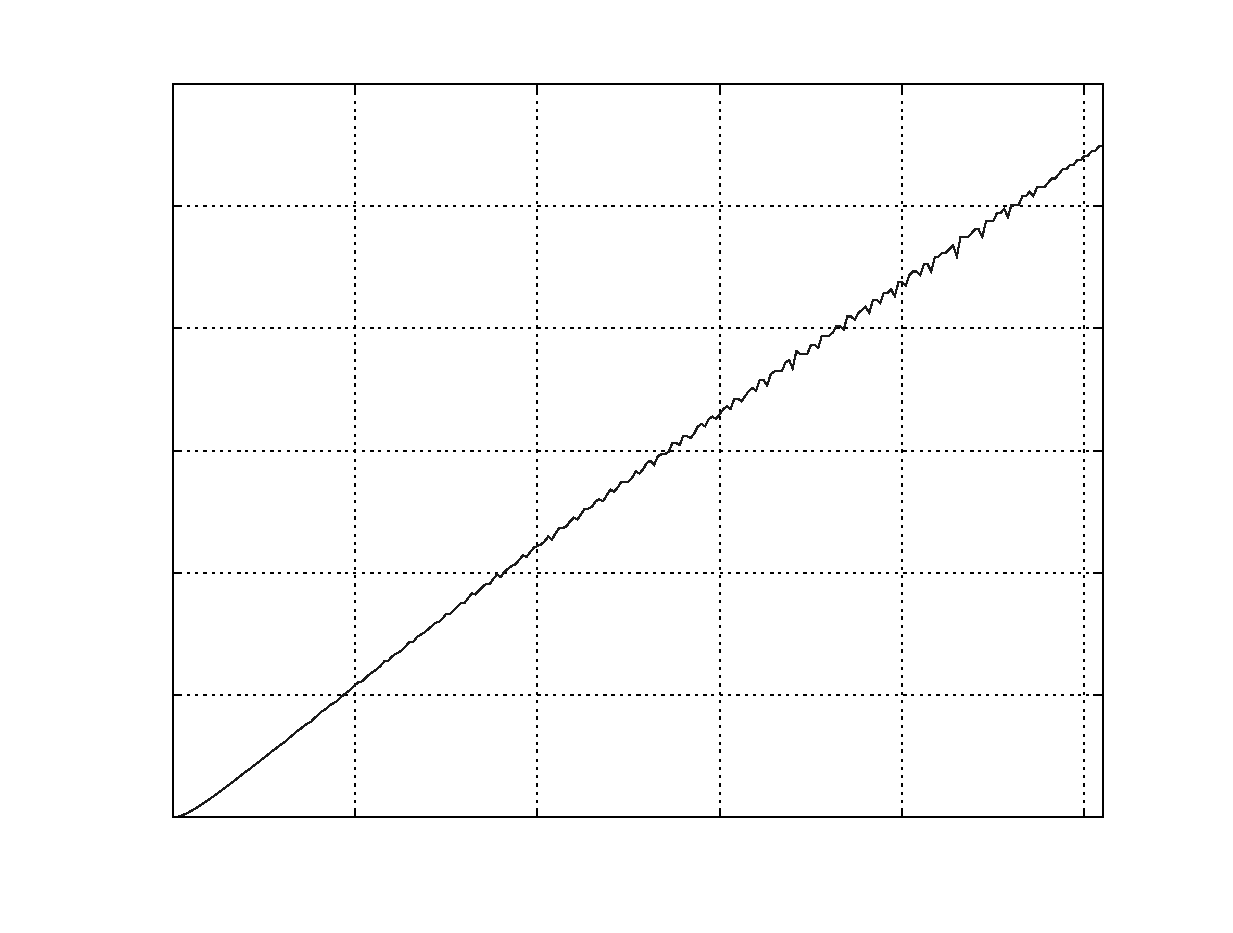
\includegraphics{img/pwm_to_lux-inc}
\end{picture}%
\begin{picture}(576,432)(0,0)
\fontsize{10}{0}
\selectfont\put(74.88,42.5189){\makebox(0,0)[t]{\textcolor[rgb]{0,0,0}{{0}}}}
\fontsize{10}{0}
\selectfont\put(162.409,42.5189){\makebox(0,0)[t]{\textcolor[rgb]{0,0,0}{{50}}}}
\fontsize{10}{0}
\selectfont\put(249.939,42.5189){\makebox(0,0)[t]{\textcolor[rgb]{0,0,0}{{100}}}}
\fontsize{10}{0}
\selectfont\put(337.468,42.5189){\makebox(0,0)[t]{\textcolor[rgb]{0,0,0}{{150}}}}
\fontsize{10}{0}
\selectfont\put(424.998,42.5189){\makebox(0,0)[t]{\textcolor[rgb]{0,0,0}{{200}}}}
\fontsize{10}{0}
\selectfont\put(512.527,42.5189){\makebox(0,0)[t]{\textcolor[rgb]{0,0,0}{{250}}}}
\fontsize{10}{0}
\selectfont\put(69.8755,47.52){\makebox(0,0)[r]{\textcolor[rgb]{0,0,0}{{0}}}}
\fontsize{10}{0}
\selectfont\put(69.8755,106.2){\makebox(0,0)[r]{\textcolor[rgb]{0,0,0}{{10}}}}
\fontsize{10}{0}
\selectfont\put(69.8755,164.88){\makebox(0,0)[r]{\textcolor[rgb]{0,0,0}{{20}}}}
\fontsize{10}{0}
\selectfont\put(69.8755,223.56){\makebox(0,0)[r]{\textcolor[rgb]{0,0,0}{{30}}}}
\fontsize{10}{0}
\selectfont\put(69.8755,282.24){\makebox(0,0)[r]{\textcolor[rgb]{0,0,0}{{40}}}}
\fontsize{10}{0}
\selectfont\put(69.8755,340.92){\makebox(0,0)[r]{\textcolor[rgb]{0,0,0}{{50}}}}
\fontsize{10}{0}
\selectfont\put(69.8755,399.6){\makebox(0,0)[r]{\textcolor[rgb]{0,0,0}{{60}}}}
\fontsize{10}{0}
\selectfont\put(298.08,31.5188){\makebox(0,0)[t]{\textcolor[rgb]{0,0,0}{{PWM value (0--255)}}}}
\end{picture}
}
    \caption{Illuminance detected by the LDR in function of the duty of the LED}
    \label{fig:pwm_to_lux}
\end{figure}

